\section{Ergebnis}
Um den Urlaubsgenehmigungsprozess zu überprüfen, haben wir die fünf verschiedene Beispielszenarien aus der Aufgabenstellung durchgespielt und im Folgenden dokumentiert.

\subsection{Szenario A}
\textit{Frau Antje beantragt 10 Tage Urlaub. Ihre Chefin genehmigt den Urlaub, es stehen noch 10 Tage Resturlaub zur Verfügung.}

\begin{figure}[H]
\centering

\includegraphics[width=1.0\linewidth]{Bilder/BeispielA}
\caption{Urlaubsgenehmigungsprozesses für Szenario A}
\label{fig:BeispielA}
\end{figure}

Der Urlaubsantrag von Frau Antje wird an ihre Vorgesetzte Frau Ennel weitergeleitet, die den Antrag genehmigt. Da noch ausreichend Resturlaubstage zur Verfügung stehen genehmigt auch der zuständige Sachbearbeiter Herr Machfrei den Antrag. Abschließend erhält Frau Antje die Benachrichtigung, dass ihr Antrag genehmigt wurde.

\subsection{Szenario B}
\textit{Herr Detuwas möchte 10 Tage Urlaub. Ihm stehen noch 20 Tage Resturlaub zur Verfügung. Nach drei Tagen hat sein Chef noch nicht reagiert.}

\begin{figure}[H]
\centering

\includegraphics[width=1.0\linewidth]{Bilder/BeispielB}
\caption{Urlaubsgenehmigungsprozess für Szenario B}
\label{fig:BeispielB}
\end{figure}

Der Urlaubsantrag von Herrn Detuwas wird seinem Vorgesetzten Herrn Dechef zugewiesen. Da dieser nach drei Tagen noch nicht reagiert hat, wird der Antrag eine Ebene höher an Frau Verkauf weitergeleitet und von ihr genehmigt. Anschließend stimmt der zuständige Sachbearbeiter Herr Machfrei aufgrund der 20 Tage Resturlaub ebenfalls zu. Abschließend wird Herr Detuwas über den genehmigten Urlaubsantrag benachrichtigt.

\subsection{Szenario C}
\textit{Herr Oberboss, der in diesem Jahr noch keinen Urlaub hatte, braucht eine Auszeit und möchte 28 Tage Urlaub, die im Vorstand gerne genehmigt werden.}

\begin{figure}[H]
\centering
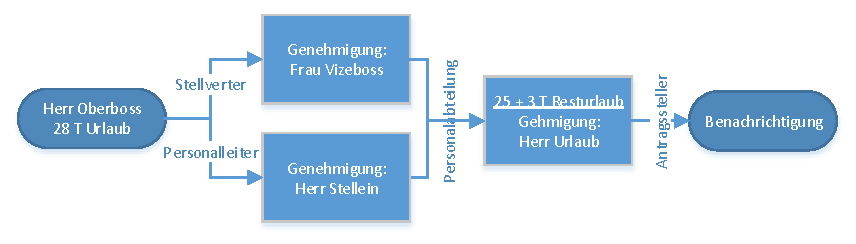
\includegraphics[width=1.0\linewidth]{Bilder/BeispielC}
\caption{Urlaubsgenehmigungsprozesses für Szenario c}
\label{fig:BeispielC}
\end{figure}

Herr Oberboss ist der Vorstandsvorsitzende. Damit muss sein Urlaubsantrag durch die stellvertretende Vorstandsvorsitzende Frau Vizeboss, die in diesem besonderen Fall die Vorgesetzte ist, genehmigt werden. Eigentlich erhalten Mitglieder des Vorstands nur 25 Tage Urlaub, allerdings wird ein Überziehen des zur Verfügung stehenden Urlaubs um maximal drei Tage geduldet. Da der Antrag mehr als 20 Tage beinhaltet, muss er zusätzlich durch Herrn Stellein, dem Leiter der Personalabteilung, genehmigt werden. Nachdem Frau Vizeboss und Herr Stellein dem Antrag zugestimmt haben, wird dieser an den zuständigen Sachbearbeiter Herrn Urlaub in die Personalabteilung weitergeleitet. Auch dieser genehmigt den Antrag, worauf Herr Oberboss benachrichtigt wird.

\subsection{Szenario D}
\textit{Kurz nach der Rückkehr aus Ihrem Urlaub zieht Frau Antje um und beantragt daher einen Tag Sonderurlaub.}

\begin{figure}[H]
\centering

\includegraphics[width=0.75\linewidth]{Bilder/BeispielD}
\caption{Urlaubsgenehmigungsprozesses Szenario D}
\label{fig:BeispielD}
\end{figure}

Da Sonderurlaubsanträge für Umzug bis zu einem Tag immer automatisch zu genehmigen sind, wird Frau Antje direkt über den genehmigten Urlaubsantrag informiert.

\subsection{Szenario E}
\textit{Herr Auchda (Resturlaub 20 Tage) beantragt 10 Tage Urlaub. Diese werden genehmigt.}

\begin{figure}[H]
\centering

\includegraphics[width=1.0\linewidth]{Bilder/BeispielE}
\caption{Urlaubsgenehmigungsprozesses Szenario E}
\label{fig:BeispielE}
\end{figure}

Da Herr Auchda ein Mitglied des Vorstands ist, muss der Vorstandsvorsitzende Herr Oberboss über den Antrag entscheiden. Dieser genehmigt den Urlaubsantrag. Anschließend wird der Antrag an den zuständigen Sachbearbeiter Herr Machfrei in die Personalabteilung weitergeleitet. Da noch genügend Resturlaub besteht wird der Antrag genehmigt und Herr Auchda erhält eine entsprechende Benachrichtigung.
